 \section{B-splines and Fitting}
 Here we only provide basic details on B-spline functions and refer the reader to 
 \cite{nurbs_book, deboor2001practical, schumaker2015spline} for further discussion. 
 Given a knot sequence $U=\left\{u_0,\ldots,u_m\right\}$ such that $u_i\leq u_{i+1},\  i=0,\ldots m-1$,
 the $i^{th}$ B-spline of degree $p$ can be defined through the recurrence formula:
 \begin{align}
 N_{i,0} &= \left\{ \begin{aligned}
                    1 \quad &\text{if } u_i\leq t\leq u_{i+1}\\
                    0 \quad &\text{otherwise }
                   \end{aligned}\right. \\
N_{i,p} &= \frac{t - u_i}{u_{i+p} - u_i}N_{i,p-1}(t) +  \frac{u_{i+p+1} - t}{u_{i+p+1} - u_{i+1}}N_{i+1,p-1}(t). 
 \end{align}
 A B-spline curve is defined as a combination of B-splines of the form:
 \begin{equation}
  C(t) = \sum_{i=0}^n N_{i,p}(t) \textbf P_i, \quad  \textbf P_i = \text{control point}.
 \end{equation}
From this definition and as shown in Figure \ref{fig:bspline_sine}, 
it is clear that the approximation degree, 
knot sequence and control polygon fully determine a B-spline curve.
\begin{figure}
 \centering
 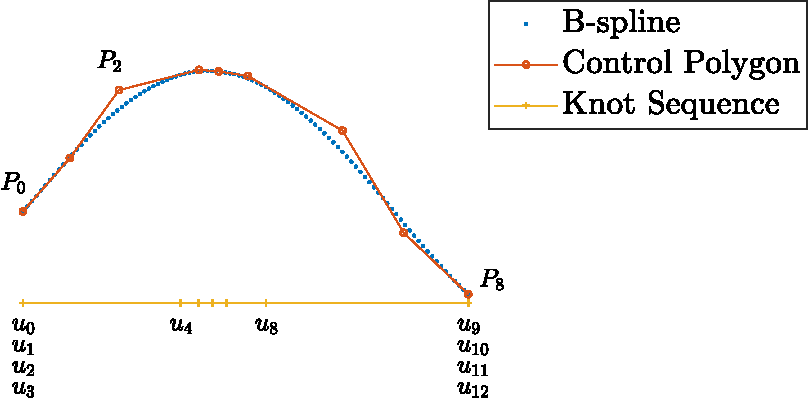
\includegraphics[width =\textwidth]{sineBspline-crop}
 \caption{\label{fig:bspline_sine} A cubic B-spline curve approximation to a piece of a sine wave employing nine
 control poinst ant the knot sequence 
 $U=\left\{u_0,\dots,u_{12}\right\}$.}
\end{figure}


\subsection{Linear Least Squares Approximation}
Given a data set $\left\{X_i\right\}_{i=1}^m$ and $n>m$ control points, 
we look for the B-spline curve 
\begin{equation}\label{eq:least_squares_equation1}
 C(t) = \sum_{i=0}^n N_{i,p}(t) \textbf P_i,\quad t\in[0,1]
\end{equation}
that approximates the data in the least squares sense:
\begin{enumerate}
 \item $ C(0)= X_0, \quad \  C(1) = X_m\quad \text{and}$
 \item $\sum _{k= 1}^{m-1}\left | X_k - C(t_k)\right|^2\quad \text{is a minimum with respect }\mathbf P_i.$
\end{enumerate}
Here the $t_k$ are associated to each data point ($X_k$) 
by a previously chosen parametrization. 

The solution to this problem can be found as follows \cite[Ch. 9.4.1]{nurbs_book}:
let 
$$
 R_k = Q_k - N_{0,p}(t_k)\cdot Q_0 - N_{m,p}(t_k)\cdot Q_m,  \quad k = 1,\ldots, m-1.
$$
Since the B-spline knots are fixed, minimizing equation \eqref{eq:least_squares_equation1} gives:
\begin{equation}\label{eq:linear_least_squares_solver}
 \sum_{i=1}^{n-1} \left(N_{\ell, p}(t_k)N_{i,p}(t_k)\right)P_i= \sum_{k=1}^{m-1}N_{\ell,[}(t_k)R_k, \quad \ell= 1\ldots, n-1
\end{equation}
 which produces a determined system of equations that can be solved applying
 any linear matrix solver. The only restrictions on the knot-sequence is the Whitney-condition:
 
The downside of a solver of this kind is that 
it assumes prior knowledge of the ``correct'' number of control points as well as the knot 
location. In order to overcome this, we propose an algorithm which strategically inserts new knots as part of an 
error controlled iterative scheme. We wish to remark that the optimization function remains linear and as a 
function of the control points only. The knot sequence increases within each iteration 
and is based on the error bisection approach presented next. 
 
\subsubsection{Knot Placement}\ref{sec:knot_placment}
A suitable knot sequence must ensure that each span contains at least one $t_k$ value so that \eqref{eq:linear_least_squares_solver} is well posed. 
We start with the minimum number of control points ($n = p$) and the following \emph{clamped} knot sequence 
$U=\{0,\underbrace{\ldots}_{p-1},0,1,\underbrace{\ldots}_{p-1},1\}$. 

 Then, at each iteration, we find the span with greatest squared error: 
 $$e_k = \frac{1}{N_k}\sum_{i=1}^{N_k} (C(t_i) - X_i)^2,\quad N_k = \# t_i\in [u_k, u_{k+1}),\ i=1,\ldots,m-1, $$
 where the distance function is computed as follows:
 \begin{equation}
  C(t_i) - X_i = \min_{t\in[0,1]} |C(t) -  X_i|,
 \end{equation}
$i.e.$, the \emph{actual} distance to the data. The new knot position is determined by
 the first $t_i$ such that $t_i >= \frac{e_k}{2}$ and taking
 the value $\tilde u = 0.5(t_i+t_{i+1})$. This knot choice ensures that the spans $[u_i, \tilde u),\ [\tilde u,u_{i+1})$ are non empty. 
Alternatively, one could find all the spans that are 
above the targeted tolerance and bisect each of them \cite[Ch. ]{nurbs_book}. 
 However, this may lead to an excessive number of control points since it does not account  
 for the fact that each span has impact in more than one control point. 
Furthermore, a span bisection does not account for the error distribution within the span nor 
the fact that it can produce empty spans. Our results suggest that a strategic knot insertion consistently improves the error as shown in Figure \ref{fig:}. 

It is well known that as the number of control points reach the number of data points ($n=m$), the spline curve might develop wiggles. 
Hence, the knot insertion process needs to be controlled so that ``locally'', the approximation process does not attempt interpolate each data point. 
This is accomplished by introducing the following constraints: the new knot has to be at a \emph{minimum} distance from its neighboring knots and initially, 
the minimum $t_k$'s per span should be set greater than one. We say initially because for sharp features with few data support, this condition may need to be relaxed in order 
to for example, detect a cusp.
 However, such artifacts may not be visible to the Least-Squares solver since curve has is smooth along the chosen parametrization 
. Figure \ref{fig:bspline_wiggle} illustrates this phenomena: the curve values that 
 are fed to the solver correspond to the centripetal parametrization (smooth) and the uniform values correspond to 
 sampling the curve uniformly around the resulting curve. 
 Observe how the Bspline wiggles in between the centripetal knots. This is because in that region, almost all the 
 knot spans contain only one $t-value$ resulting in a zig-zagging control polygon.


the resulting approximating B-spline curve may develop undesirable wiggles or artificial loops (self-intersections). 
 
 
 \begin{figure}
  
  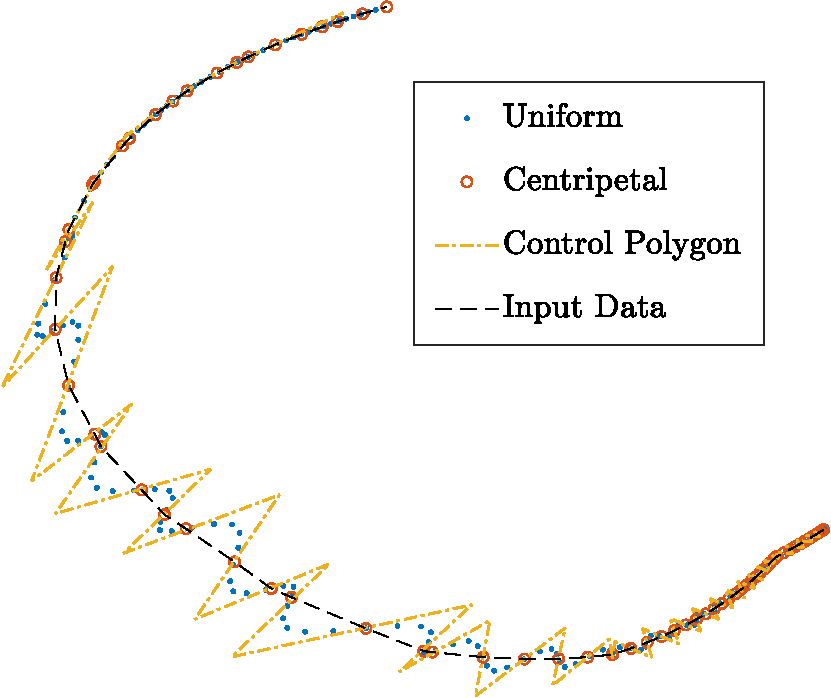
\includegraphics{wiggle_ALL-crop}
  \caption{\label{fig:bspline_wiggle}Bspline approximation sampled at two different parametrizations (centripetal and uniform) revealing the ``hidden'' wiggles as a result excessive number 
  of control points.}
 \end{figure}


\subsubsection{The Algorithm}
Now that the least squares approach and knot placement have been discussed, we introduce the main algorithm and discuss implementation 
details. Once the desired tolerance is selected, we use the centripetal method in order to obtain a curve parametrization: 
\begin{align}
 d &= \sum_{k=1}^n \sqrt {| X_k-X_{k-1}|},\\
 t_0 &=0,\ t_m=1,\quad t_k = t_{k-1} + \frac{\sqrt{|X_k-X_{k-1}|}}{d},\quad k = 1,\ldots, m-1.
 \end{align}
This method has proven to be suitable for detecting curve features such as ``cusps'' \cite{}. 
\begin{note}
 If the initial number of control points is set $n > p$, we define the internal knots sequence proposed by proposed by \cite{}: 
  \begin{align}
  d &= \frac{m+1}{n-p+1} \Rightarrow i = int(j\cdot d),\quad \alpha = jd -i\\
  u_{p+j} &= (1-\alpha)u_{i-1} + \alpha u_i,\quad j = 1,\ldots,n-p.
 \end{align}
\end{note}

At each iteration, we solve \eqref{} and compute the global error. If we haven't reached the desired tolerance, 
we insert a knot as discussed in section \ref{sec:knot_placment} and find the new control points. If the 
new configuration has not significantly improved the previous iteration, we reject the knot and find the next worst error. 
 If all knots were found to be ``unsuitable'' we proceed with the best configuration, insert a new knot and tag its 
 value. Once a significant improvement has been found, we try to remove all the ``redundant'' points computed between the tagged knot and the 
 knot at valid iteration and when possible, the knots in between are removed. The algorithm stops when either the tolerance has reached, 
 the number of iterations have exceeded the maximum or when the approximation has stagnated: no new knot 
 produces a better approximation. The implementation steps are shown in Algorithm \ref{alg:solver}. 

 
 
 \section{The Algorithm}
 
 The work presented here provides a solution to data approximation in the least-squares sense through an iterative 
 scheme that aims to attain a user specified accuracy. 
In order to avoid solving the non-linear ``free knots'' problem, we propose the following approach: start with few (or minimal) number of control points and perform a curve fit solving the linear least-squares problem in order to find 
the points location. If the error is unacceptable, locate the knot span with highest squared error and insert a  new knot such that the error is split in halves. The process iterates until the desired tolerance is reached or it is not 
possible to introduce new suitable knots. We will discuss later what unsuitable knots mean. 


 
 
 are not visible to the 
Hence, we believe that 
a ``knot increasing'' iterative scheme is more stable than approximating the curve starting with a high number of control points and iterative remove the redundant ones. 
The usual approach for solving the least squares problem consists of a pre-stage that finds a suitable curve parametrization ($e.g.$, centripetal or chord-length)  ${t_j}_{j=1}^m$ that targets the $m$ data points and
then compute the knots location followed by finding the control points location that minimizes the error in the least squares sense. 
This curve discretization does observe the curve behavior between the evaluations $B(t_j)$ and $B(t_{j+1})$, where a ``parasitic'' loop may develop. If the local error is smaller than the tolerance, that 
curve zone will not be altered ($i.e.$, candidate for knot-removal in a knot decreasing iterative scheme) thus, producing undesirable results. Furthermore, knot spans that contain few $t$-values can end up having a dense control point area 
producing wiggles. Again, from the least-squares perspective, such wiggles do not exist as illustrated in Figure \ref{fig:wiggle_unif_vs_centr}.



\subsubsection{Computational Costs}
The methodology presented here attempts to avoid the ``free knot problem'' which involves solving a non-linear 
least squares solver. By sequentially increasing the number of control points together with a well chosen knot 
position, we can obtain a suitable approximation which relies on solving a linear system thus, avoiding excessive 
computational costs. Although we cannot prove that our knot position is optimal, it is designed to increase the accuracy 
 at where the maximum error in the least squares sense occur,
  thus it is in accordance with the minimization solver. 
  Furthermore as shown in the next section, our results reveal that this routine is suitable for 
   noisy data and does not ``destroy`` sharp features. 
   
   
\section{Results}
We begin by studying the performance of the solver on ''basic shapes`` as well as smooth data. 
Then we apply this routine on a level-set solution employed for studying ice formation and finally, we study 
 its behavior on nosy data. 
 

 \begin{table}
 \centering
  \begin{tabular}{||c||c c || c c ||}
  \hline
 R.M.S.  &\multicolumn{4}{c||}{Control Points}\\
 \hline
  &\multicolumn{2}{c||}{\textbf{Sphere Curve}} & \multicolumn{2}{c||}{\textbf{NACA}}\\

 TOL& ECILS& DLS & ECILS & DLS\\
 \hline
1.0e-05 & 30 & 22 & 10 & 19 \\%& 33 & 67\\
1.0e-06 & 52 & 36 & 19 & 35 \\%& &\\
1.0e-07 & 84 & 60 & 42 & 54 \\%& &\\

\hline
&\multicolumn{2}{c||}{}&\multicolumn{2}{c||}{}\\
&\multicolumn{2}{c||}{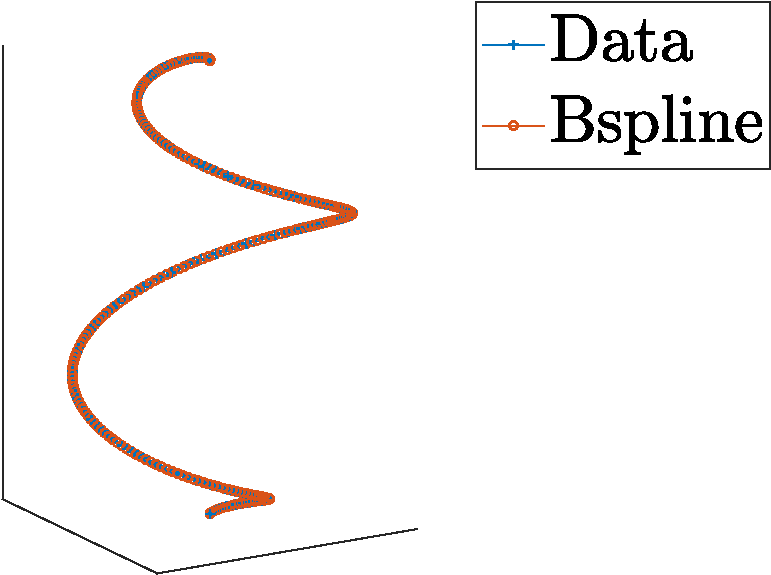
\includegraphics[width=0.42\textwidth]{snake-crop}}
&\multicolumn{2}{c||}{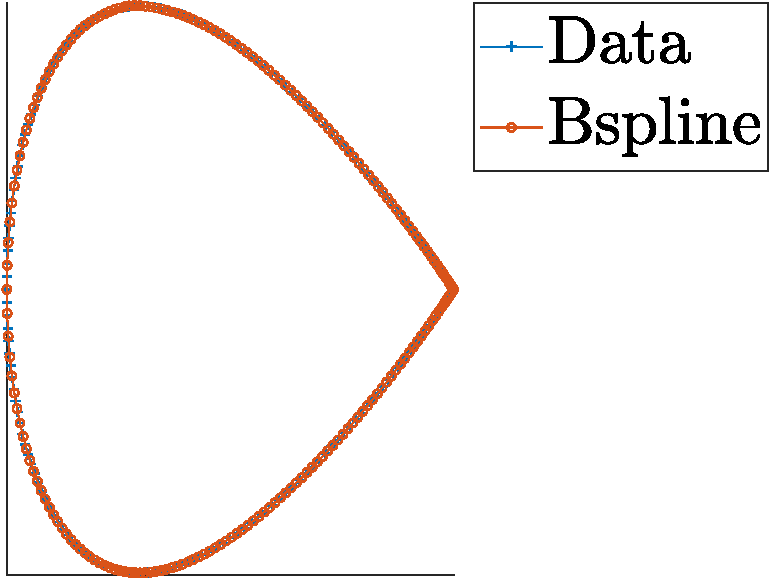
\includegraphics[width=0.42\textwidth]{naca27-crop} }\\
\hline
\end{tabular}
\caption{Results when approximating a curve moving along a sphere (see Figure \ref{fig:sphere_snake}) using 200 points.}
 \end{table}

 
 
 
 \begin{figure}
  \begin{tabular}{ccc}
  \hline
{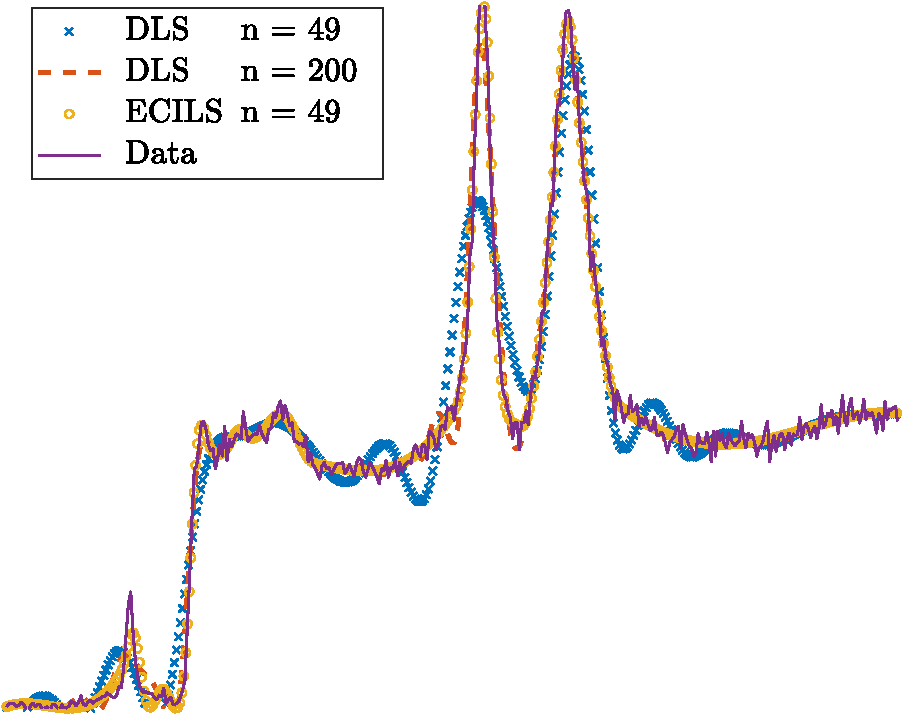
\includegraphics[width=0.29\textwidth]{noise1}}
&{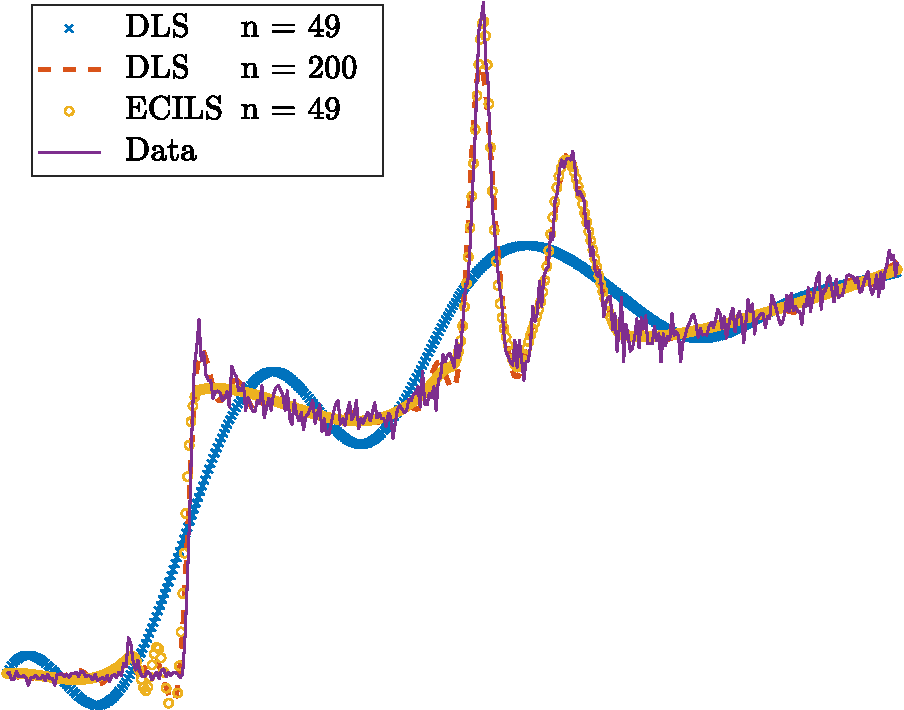
\includegraphics[width=0.29\textwidth]{noise2}}
&{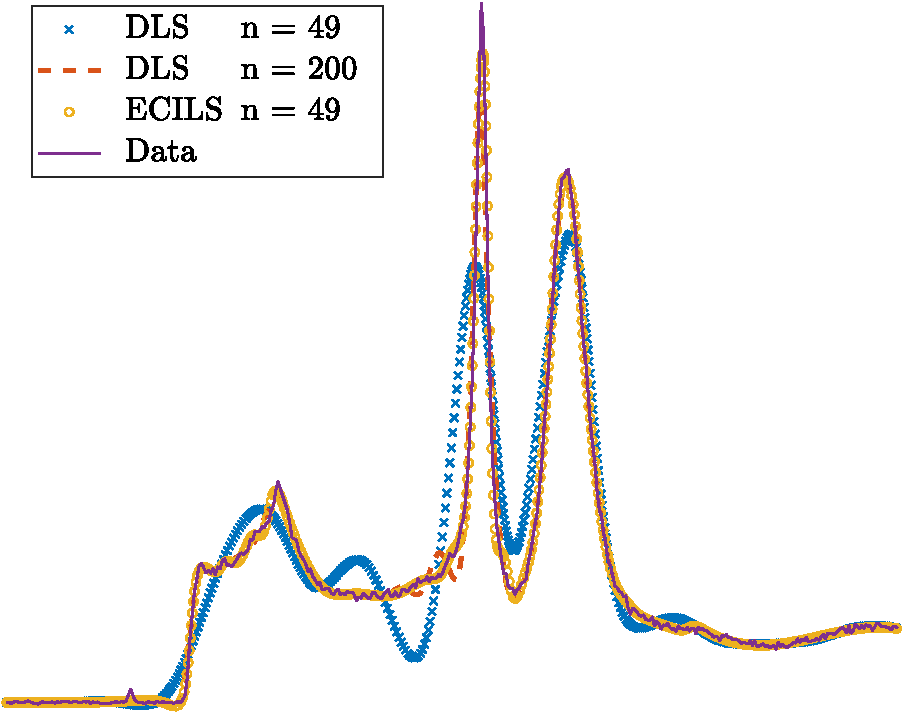
\includegraphics[width=0.29\textwidth]{noise3}}\\
\hline
  \end{tabular}
\caption{\label{fig:noise_DLS_vs_ECILS} Three data samples from Raman Spectroscopies (*) 
and the resulting approximation using the new algorithm versus a direct fit for different number of control points. 
}
 \end{figure}



 
 Figure \ref{} shows a helix obtained from \subsection{Basic Shapes Approximation}
 Consider
 
 



   
